\documentclass[11pt]{article}

% ---- packages ----
\usepackage[margin=1in]{geometry}
\usepackage{graphicx}
\usepackage{booktabs}
\usepackage{amsmath}
\usepackage{caption}
\usepackage{microtype}
\usepackage[hidelinks]{hyperref}
\usepackage{titlesec}
\usepackage{authblk}

\captionsetup{font=small,labelfont=bf}
\titleformat{\section}{\large\bfseries}{\thesection}{0.6em}{}
\titleformat{\subsection}{\normalsize\bfseries}{\thesubsection}{0.6em}{}
\setlength{\parskip}{0.4em}
\setlength{\parindent}{0pt}

\title{\bfseries Engineering Radiotrophic Metabolism in Human Cells:\\
A Constraint-Based Feasibility Analysis}
\author{Adam Labban}
\date{Preprint draft. Computational feasibility study; results are in silico
and not experimentally validated (see Section~\ref{sec:limitations}).}

\begin{document}
\maketitle

\begin{abstract}
\noindent
Melanized fungi colonizing high-radiation environments such as the Chernobyl
reactor appear to use ionizing radiation as a metabolic resource, a phenomenon
termed radiotrophy. Whether the same capacity could be engineered into human
cells is unknown. Here we ask a deliberately narrow question: not whether
radiotrophy could out-compete glucose metabolism, but whether a human cell could
be engineered to treat ionizing radiation as a usable, survivable energy input
rather than purely as damage. We built a constraint-based (flux-balance)
metabolic model of a human cell (56 reactions, 52 metabolites) augmented with a
melanin-driven radiotrophic NADH-generating pathway and a layered set of native
and cross-species engineered reactive-oxygen-species (ROS) defenses (superoxide
dismutase, catalase, glutathione peroxidase, tardigrade Dsup, \textit{Deinococcus}
Mn-antioxidant, Nrf2, and overexpressed MnSOD2). Under a forced-dose protocol, in
which the cell cannot decline the radiation it absorbs, the model produces a clear
three-regime response: a RESOURCE regime in which radiation yields net ATP with
the radical load fully neutralized and zero net DNA damage; a STRAINED regime in
which defenses saturate, DNA lesions accrue, and net ATP declines while remaining
positive; and a LETHAL regime in which no feasible metabolic steady state exists
(cell death). Defense-ablation analysis identifies superoxide dismutase and
glutathione-mediated radical scavenging as the two single points of failure, and
a targeted analysis shows that superoxide, not hydroxyl radical, is the species
that overwhelms the cell first, because hydroxyl damage can be paid down through
ATP-dependent repair whereas superoxide has only the capacity-limited SOD exit.
The qualitative result is robust to the most uncertain model parameter. These
findings frame a concrete, testable hypothesis and an engineering priority list
(chiefly SOD augmentation), and we propose a wet-lab experiment designed to
isolate energy capture from radioprotection. We emphasize that the model's
radiation axis is not physically dimensioned and that no claim here has been
experimentally validated.
\end{abstract}

\section{Introduction}

Ionizing radiation is, for essentially all human cells, a pure liability: it
generates reactive oxygen species and DNA lesions, drives mutagenesis, and at
sufficient dose causes death. Yet certain melanized fungi not only tolerate
intense radiation but appear to grow better under it. Isolates recovered from the
walls of the damaged Chernobyl reactor, and later flown on the International Space
Station, show enhanced growth under elevated radiation, an effect linked to their
melanin content \cite{dadachova2007,shunk2022}. The proposed mechanism,
radiotrophy, is that melanin acts as a broadband absorber that transduces
radiation energy into a usable form, increasing the reducing capacity (NADH)
available to metabolism \cite{dadachova2007,turick2011}.

The remarkable claim of radiotrophy is not that it is an efficient energy source.
It is not, and melanized cells do not outgrow well-fed controls on rich media. The
remarkable claim is qualitative: that radiation, normally a hazard, can serve as a
metabolic input at all. For human cells the corresponding question is sharper
still, because a baseline human cell has no positive use for radiation whatsoever.
Could one engineer a human cell in which radiation becomes net-tolerable, even
net-beneficial, instead of strictly destructive?

This question sits at the intersection of two literatures that have so far
remained largely separate. The first is radioprotection: melanin shielding, the
tardigrade damage-suppressor protein Dsup \cite{hashimoto2016,chavez2019}, the
\textit{Deinococcus radiodurans} manganese-antioxidant system \cite{daly2004}, and
antioxidant-pathway activation \cite{lewis2015} all reduce radiation harm and are,
individually, well established. The second is radiotrophy: energy capture from
radiation, demonstrated phenomenologically in fungi but mechanistically contested.
Combining them, asking whether a human cell could both survive radiation and
harvest energy from it, has not, to our knowledge, been modeled.

We formalize the question with two hypotheses:
\begin{itemize}
  \item \textbf{Null (H$_0$):} Radiation is a strict liability for an engineered
  human cell; any energy captured by melanin is outweighed by the ROS and DNA
  damage it generates, so the cell is no better off, or dies.
  \item \textbf{Alternative (H$_1$):} Melanin plus engineered ROS defenses allow a
  human cell to route radiation energy into ATP while keeping the resulting damage
  survivable, up to some dose ceiling.
\end{itemize}

We test these with a constraint-based metabolic model. Constraint-based modeling
is well suited to a feasibility question: it asks what a metabolic network can do
at steady state under stoichiometric and capacity constraints, without requiring
kinetic parameters that are unavailable for an organism that does not yet exist.
We stress at the outset that this is an in silico feasibility study: it can show
that a hypothesis is internally consistent and worth testing, not that it is true
of real cells.

\section{Methods}

\subsection{Model construction}

The model is a constraint-based reconstruction built with COBRApy, comprising 56
reactions and 52 metabolites across three compartments (cytosol, mitochondrion,
extracellular). Core energy metabolism is represented by lumped glycolysis, a full
tricarboxylic-acid cycle, and a lumped electron transport chain with a
physiological P/O ratio and a small (approximately 1\%) electron leak to
superoxide. Melanin biosynthesis is modeled from tyrosine via tyrosinase and a
lumped melanin-synthesis reaction. The objective is ATP maintenance (a non-growth
ATP demand), maximized by flux-balance analysis.

\subsection{The radiotrophic pathway and ROS production}

The novel reaction, RADIO, represents melanin-mediated transduction of radiation
into reducing power: it consumes melanin and NAD$^{+}$ and produces NADH, with
reactive oxygen species as obligate byproducts. Per unit RADIO flux it generates
0.28 superoxide and 0.24 hydroxyl radical; these coefficients derive from
water-radiolysis G-values \cite{buxton1988} adjusted for partial melanin quenching
\cite{schweitzer2009}, and a small ATP overhead per NADH represents the cost of
energy transduction, consistent with the ATP decline reported by Bryan et al.\
\cite{bryan2011}. The ROS-per-flux constants are enforced to match the reaction
stoichiometry by a build-time assertion, so they cannot silently drift.

\subsection{ROS defenses}

Native defenses (superoxide dismutase, catalase, glutathione peroxidase and
reductase, glutathione-mediated hydroxyl scavenging) are capacity-capped to finite
physiological pools. Cross-species engineered defenses are added as modular
reactions: the tardigrade Dsup protein (hydroxyl interception at chromatin), the
\textit{Deinococcus} Mn-antioxidant complex, an enhanced Nrf2 glutathione-recycling
pathway, and overexpressed MnSOD2.

Two constraints encode the key biology. First, Dsup is capped at intercepting at
most 40\% of generated hydroxyl radicals, matching the approximately 40\%
DNA-damage reduction measured by Hashimoto et al.\ \cite{hashimoto2016}, via a
coupling constraint linking Dsup flux to RADIO flux; without it, flux-balance
optimization routes 100\% of radicals through the near-free Dsup reaction and pays
no DNA-repair cost, overstating its benefit. Second, glutathione scavenging is
given a finite capacity, so that beyond it hydroxyl radicals must either be
intercepted by Dsup or become DNA lesions repaired by base-excision repair at a
cost of approximately 4 ATP per lesion \cite{lindahl2000}. This finite cap is what
allows DNA damage to occur at high dose, making the survival question testable
rather than assumed away. The overall mechanism is summarized in
Figure~\ref{fig:mechanism}.

\subsection{Forced-dose protocol}

A cell in a radiation field cannot decline the dose it absorbs. To represent this,
the central experiment fixes RADIO flux to a series of values (rather than letting
the optimizer choose it) and asks, at each: how much net ATP is produced relative
to zero dose; how the radical load partitions among interception, scavenging, and
DNA lesions; and whether any feasible steady state exists at all. Infeasibility is
interpreted as the cell being unable to balance the radical load, that is, death.

\subsection{Reproducibility}

The linear-program solver is pinned to GLPK (deterministic), all model parameters
are named constants, and dependency versions are pinned. Outputs are byte-identical
across runs, and a suite of eight invariant tests guards the central findings
(baseline ATP, the Dsup 40\% cap, finite scavenging, the three-regime arc, the SOD
single-point-of-failure, and determinism). All code and data are released.

\subsection{Dose calibration (illustrative only)}
\label{sec:calibration}

We attempted to convert the model's flux axis to absorbed dose (Gray) using
radiolysis G-values. This first-principles calibration overshoots realistic lethal
doses by approximately $10^{6}$, confirming that the model's fluxes are relative,
not physically dimensioned. We therefore report an explicitly illustrative,
anchored scale, matching the model's lethal threshold to a representative acute
mammalian lethal dose (approximately 10 Gy); absolute Gy values in figures are
approximate analogies, not measurements.

\section{Results}

\subsection{Radiation as a survivable energy source: the three-regime response}

Under the forced-dose protocol, the model produces a characteristic three-regime
response (Figure~\ref{fig:dose}):
\begin{itemize}
  \item \textbf{RESOURCE} (low dose): ATP production rises monotonically with dose,
  the radical load is 100\% neutralized, and no DNA lesions occur. Net ATP gain
  relative to the unirradiated baseline (111.4) reaches $+4.3$ at the ceiling (peak
  ATP approximately 115.8). Here radiation is unambiguously a usable, harm-free
  energy input.
  \item \textbf{STRAINED} (intermediate dose): defenses saturate. The fraction of
  radicals neutralized falls (to approximately 85\% at the upper end), DNA lesions
  appear and are repaired at ATP cost, and net ATP declines but remains positive.
  Radiation is still net-beneficial, but increasingly costly.
  \item \textbf{LETHAL} (high dose): no feasible metabolic steady state exists. The
  ROS load cannot be balanced, which we interpret as cell death.
\end{itemize}

This arc is the central result: it shows that, within the model, radiation can be a
net-positive, survivable input up to a defense-limited ceiling, beyond which it
becomes first costly and then fatal. On the illustrative anchored scale, the
ceiling and lethal threshold correspond to roughly 7 and 10 Gy respectively (with
the strong caveat of Section~\ref{sec:calibration}).

\subsection{Radiotrophy as a survival supplement under nutrient stress}

The relative benefit of radiotrophy grows under energy limitation. At standard
glucose and oxygen, the radiotrophic cell gains approximately 4\% ATP over a
non-radiotrophic control; under combined glucose/oxygen restriction this rises to
approximately 12\%. Most strikingly, under zero glucose the non-radiotrophic cell
produces no ATP while the radiotrophic cell continues to produce a substantial
amount (approximately 29 flux units at moderate oxygen), that is, it subsists on
radiation alone. This positions radiotrophy as a survival supplement that matters
most precisely when conventional metabolism fails, consistent with the environments
where natural radiotrophs are found.

\subsection{Superoxide dismutase and glutathione scavenging are single points of
failure}

Systematically knocking out each defense (Figure~\ref{fig:ablation}) shows that
radiotrophy is robust to loss of most individual defenses: removing the
Mn-antioxidant complex, Nrf2, or catalase has no effect on the achievable ceiling,
and removing Dsup merely reduces it (from approximately 21 to approximately 12.5
flux). Two knockouts, however, collapse radiotrophy entirely: superoxide dismutase
and glutathione-mediated hydroxyl scavenging. Each is a single point of failure.
This identifies the load-bearing components of the engineered system and, by
extension, the highest-priority targets for any engineering effort.

\subsection{Superoxide, not hydroxyl radical, overwhelms the cell first}

Given that both superoxide and hydroxyl are produced, which one sets the lethal
threshold? A targeted analysis is decisive: augmenting superoxide handling (adding
MnSOD2) raises the lethal threshold from a flux of 29 to 59, nearly doubling the
survivable dose, whereas a twentyfold increase in glutathione scavenging capacity
leaves it unchanged. Superoxide is the species that overwhelms the cell first. The
reason is structural rather than quantitative: hydroxyl radicals possess an escape
valve, since unneutralized hydroxyl becomes DNA damage that is repaired at ATP
cost, a route that is always available, whereas superoxide's only exit is the
capacity-limited SOD reaction. Once superoxide production exceeds total SOD
capacity, no steady state exists. This makes SOD augmentation the single most
valuable intervention for raising the survivable dose, and it is annotated in the
mechanism schematic (Figure~\ref{fig:mechanism}).

\subsection{Relieving the binding bottleneck lifts the ceiling}

Because the radiotrophic ceiling is set by radical-neutralization capacity, the
correct engineering levers are those that relieve it (Figure~\ref{fig:bottleneck}).
Adding MnSOD2 alone produces no improvement, confirming that SOD is not the binding
constraint at the baseline ceiling, whereas relieving glutathione (OH-neutralization)
capacity lifts the ceiling from approximately 21 to approximately 29 flux.
Relieving both ROS bottlenecks together raises it to approximately 42, and a
combined intervention (expanded scavenging, MnSOD2, and synthetic melanin loading
to bypass the biosynthetic cost) reaches approximately 69 flux with ATP rising to
approximately 151. The lesson is that interventions must target the binding
constraint: the same MnSOD2 that is useless at baseline becomes essential once
scavenging is relieved and superoxide becomes limiting.

\subsection{The result is robust to the most uncertain parameter}

The superoxide-per-NADH coefficient is the least-constrained parameter in the
model. Varying it across a 40-fold range (Figure~\ref{fig:ros}) leaves the
qualitative conclusion intact: the net ATP gain from radiation remains positive
across the entire range, including the literature-derived band. DNA lesions appear
only at the low-cost end, where high radiotrophic flux drives damage. The central
claim, that radiation can be a net-positive, survivable input, does not depend on
the precise value of the most uncertain parameter.

\section{Discussion}

Taken together, the results support the alternative hypothesis within the model: an
engineered human cell can, in silico, treat radiation as a usable and survivable
energy input rather than as pure damage, up to a defense-limited dose. The
contribution is threefold. First, it reframes radiation for engineered human cells
from a strictly-harmful agent to a conditional resource, and makes that reframing
quantitative through the RESOURCE/STRAINED/LETHAL arc. Second, it identifies the
load-bearing biology: radical-neutralization capacity, with superoxide dismutase as
the component that sets the survival ceiling and glutathione scavenging as a
co-essential second bottleneck. Third, it yields a concrete engineering priority
list, SOD/MnSOD2 augmentation first and then glutathione capacity, that differs
from what an intuition built on radioprotection alone (for example, a focus on
Dsup) would suggest.

The model's relationship to existing experimental data is consistent under the
correct framing (Table~\ref{tab:validation}). The ISS \textit{Cladosporium} growth
advantage (approximately 21\%; \cite{shunk2022}) is of the same order as the
model's stress-condition benefit. The ATP decline reported in melanized cells at
high dose \cite{bryan2011} corresponds to the model's STRAINED-to-LETHAL transition
rather than contradicting it. The Dsup 40\% protection \cite{hashimoto2016} is
imposed directly. Crucially, the model does not reproduce the large fungal CFU
boosts \cite{dadachova2007}, and should not, since those reflect growth and repair
processes outside a steady-state ATP model, and the present thesis is about
tolerance and capture, not boost magnitude.

Among the engineered components, Dsup is the most feasible single gene transfer
(Table~\ref{tab:genes}): it has been expressed in human cells with confirmed
nuclear localization and DNA protection, targets a universally conserved nucleosome
surface, and requires no cofactors. Notably, however, the model shows Dsup is
protective but not energy-determining: it raises DNA integrity but does not set the
survival ceiling, which superoxide does. The components that most extend survivable
dose (SOD systems) are different from the one with the cleanest prior validation
(Dsup), a tension worth keeping in view for experimental design.

\section{Limitations}
\label{sec:limitations}

These results must be read with several hard limitations.
\begin{enumerate}
  \item \textbf{The radiation axis is not physically dimensioned.} Model fluxes are
  relative; the first-principles calibration fails by approximately $10^{6}$.
  Absolute Gy values are illustrative anchors, not measurements, and no quantitative
  dose claim should be drawn from them.
  \item \textbf{No experimental validation.} Every result is in silico. Comparisons
  are to third-party literature, not to experiments performed here. The model is a
  hypothesis generator, not evidence about real cells.
  \item \textbf{The model is bespoke and simplified.} Glycolysis, the ETC, and
  melanin synthesis are lumped; several ROS and melanin stoichiometries are
  literature-guided estimates rather than measured values. It is not a validated
  genome-scale reconstruction.
  \item \textbf{``Lethal'' means ``no feasible steady state.''} This is a reasonable
  proxy for death but not a calibrated survival curve, and flux-balance analysis
  omits dynamics, transient damage spikes, protein and membrane oxidation, and
  chronic effects.
  \item \textbf{The underlying premise is itself debated.} Whether melanin
  radiotrophy yields usable metabolic energy (versus radioprotection alone) is not
  settled even in fungi; the engineering hypothesis inherits that uncertainty.
\end{enumerate}

\section{Conclusion and future work}

We have shown, in a constraint-based model, that melanin-based radiotrophy combined
with engineered antioxidant defenses could allow a human cell to treat ionizing
radiation as a usable, survivable energy input up to a defense-limited dose, beyond
which superoxide overwhelms its dismutase capacity and sets a hard survival
ceiling. The result is internally consistent, robust to the most uncertain
parameter, and yields a specific engineering priority (SOD/MnSOD2 first).

The decisive next step is experimental. We outline a proof-of-concept design built
around isolating energy capture, the novel claim, from radioprotection, which is
already established. The core is a melanin $\times$ radiation $\times$ glucose
factorial in which only the radiotrophic hypothesis predicts a radiation- and
melanin-dependent ATP rescue under energy limitation; a shielded-sham control and a
synthetic-melanin arm isolate the effect, and a clean negative result would itself
meaningfully constrain the hypothesis. Beyond that, re-grounding the network in a
validated genome-scale human reconstruction and a physical dose calibration would
convert the present qualitative claims into quantitative ones.

% ---------------- FIGURES ----------------

\begin{figure}[t]
  \centering
  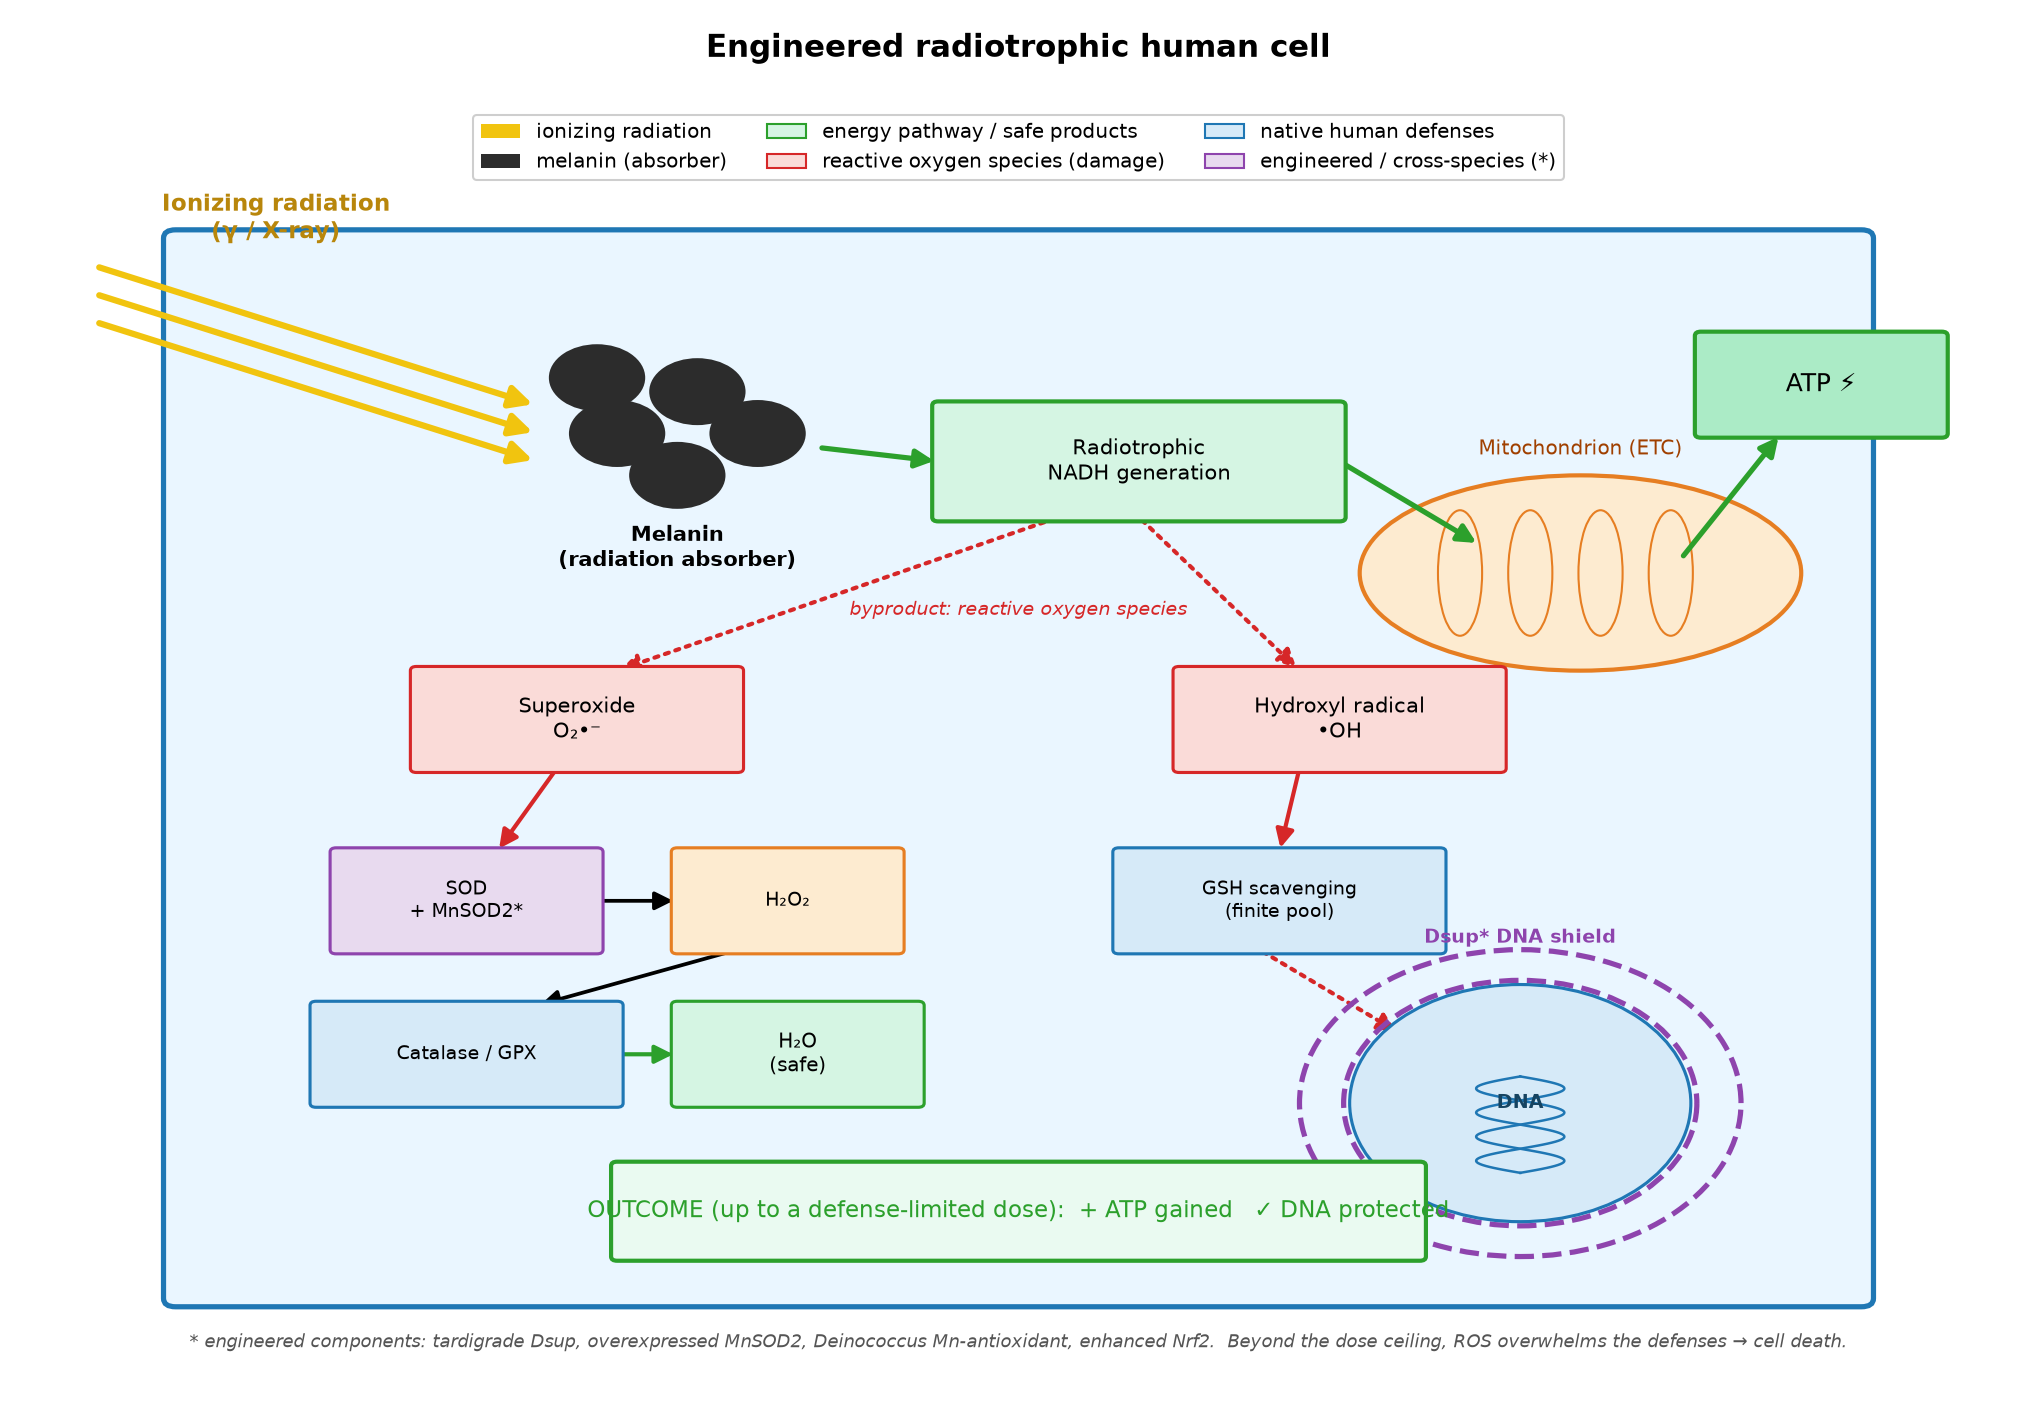
\includegraphics[width=0.92\linewidth]{fig_mechanism.png}
  \caption{Mechanism schematic. Radiation is absorbed by melanin, driving
  radiotrophic NADH generation and mitochondrial ATP synthesis. Reactive oxygen
  species (superoxide, hydroxyl radical) are obligate byproducts and are routed
  through native and engineered defenses to protect DNA up to a defense-limited
  dose. The superoxide/SOD branch is marked as the failure-first pathway.}
  \label{fig:mechanism}
\end{figure}

\begin{figure}[t]
  \centering
  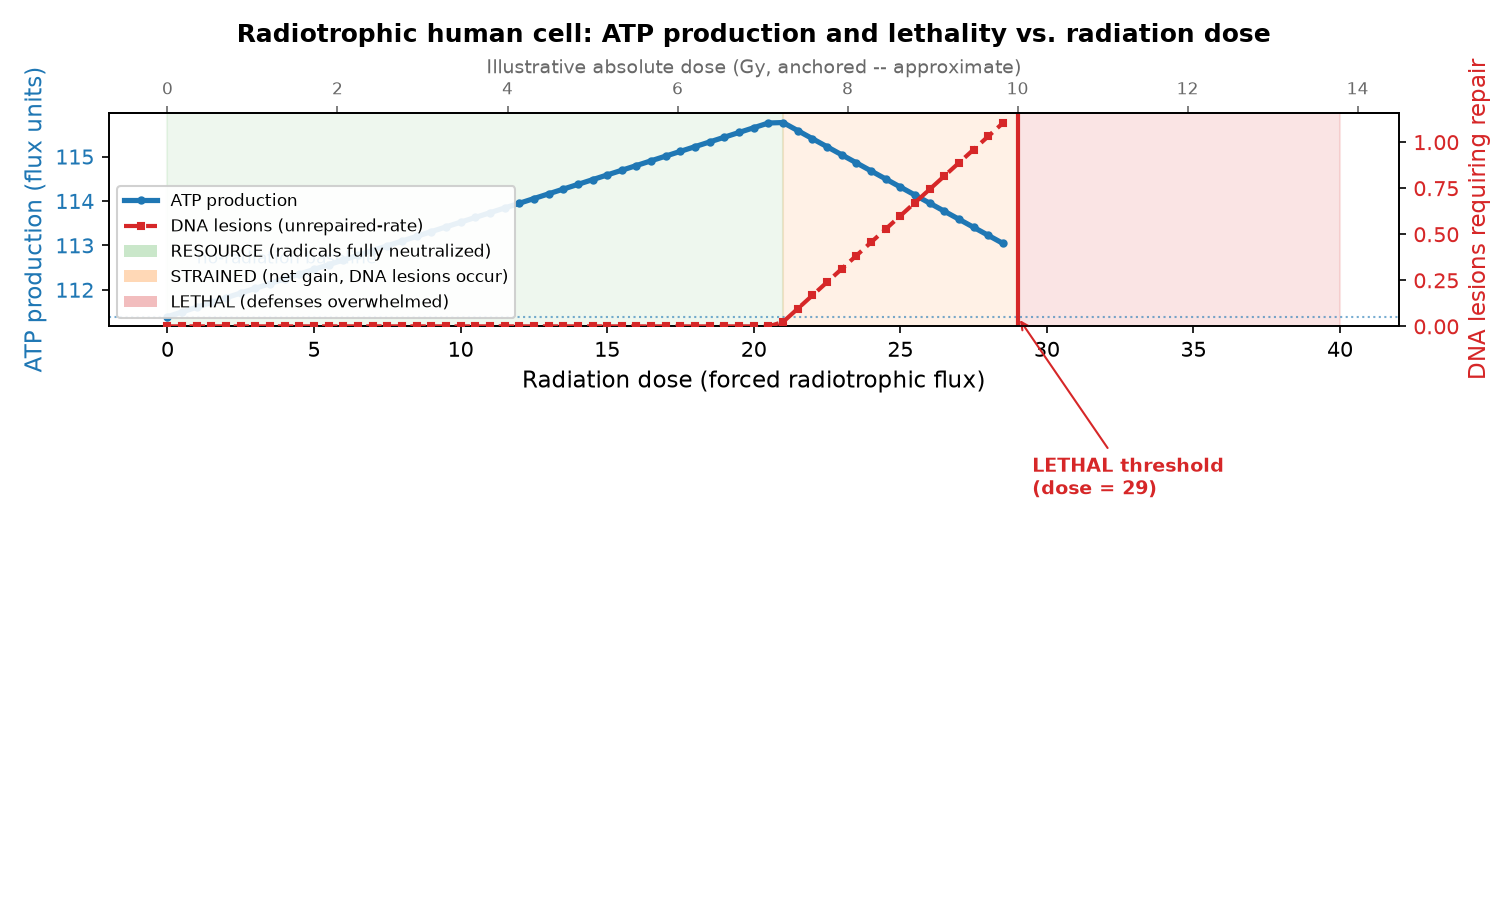
\includegraphics[width=0.92\linewidth]{radiation_atp_lethality.png}
  \caption{ATP production (blue) and DNA lesions (red) versus forced radiation
  dose, showing the RESOURCE, STRAINED, and LETHAL regimes. ATP rises while the
  radical load is fully neutralized, peaks at the defense-limited ceiling, declines
  as DNA repair consumes ATP, and terminates at the lethal threshold where no
  feasible steady state exists. Top axis: illustrative anchored dose (approximate).}
  \label{fig:dose}
\end{figure}

\begin{figure}[t]
  \centering
  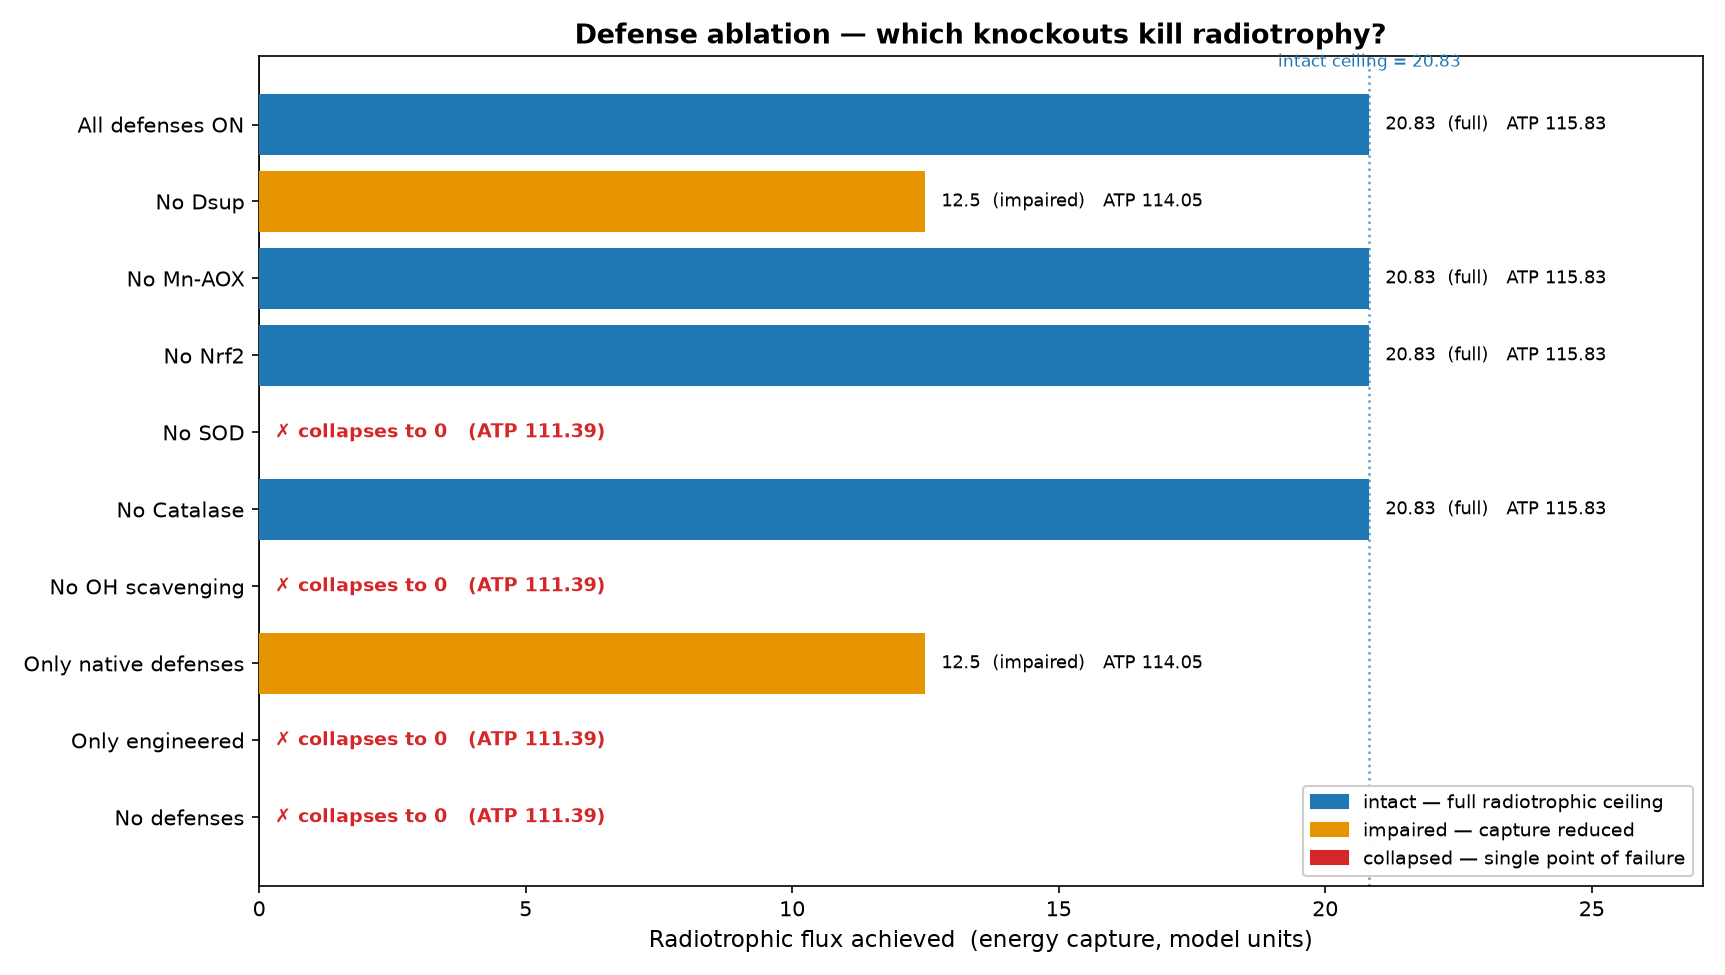
\includegraphics[width=0.92\linewidth]{fig_ablation.png}
  \caption{Defense ablation. Radiotrophic flux achieved when each defense is removed.
  Superoxide dismutase and glutathione-mediated scavenging are single points of
  failure (capture collapses to zero); Dsup loss is merely impairing; loss of the
  Mn-antioxidant, Nrf2, or catalase has no effect on the ceiling.}
  \label{fig:ablation}
\end{figure}

\begin{figure}[t]
  \centering
  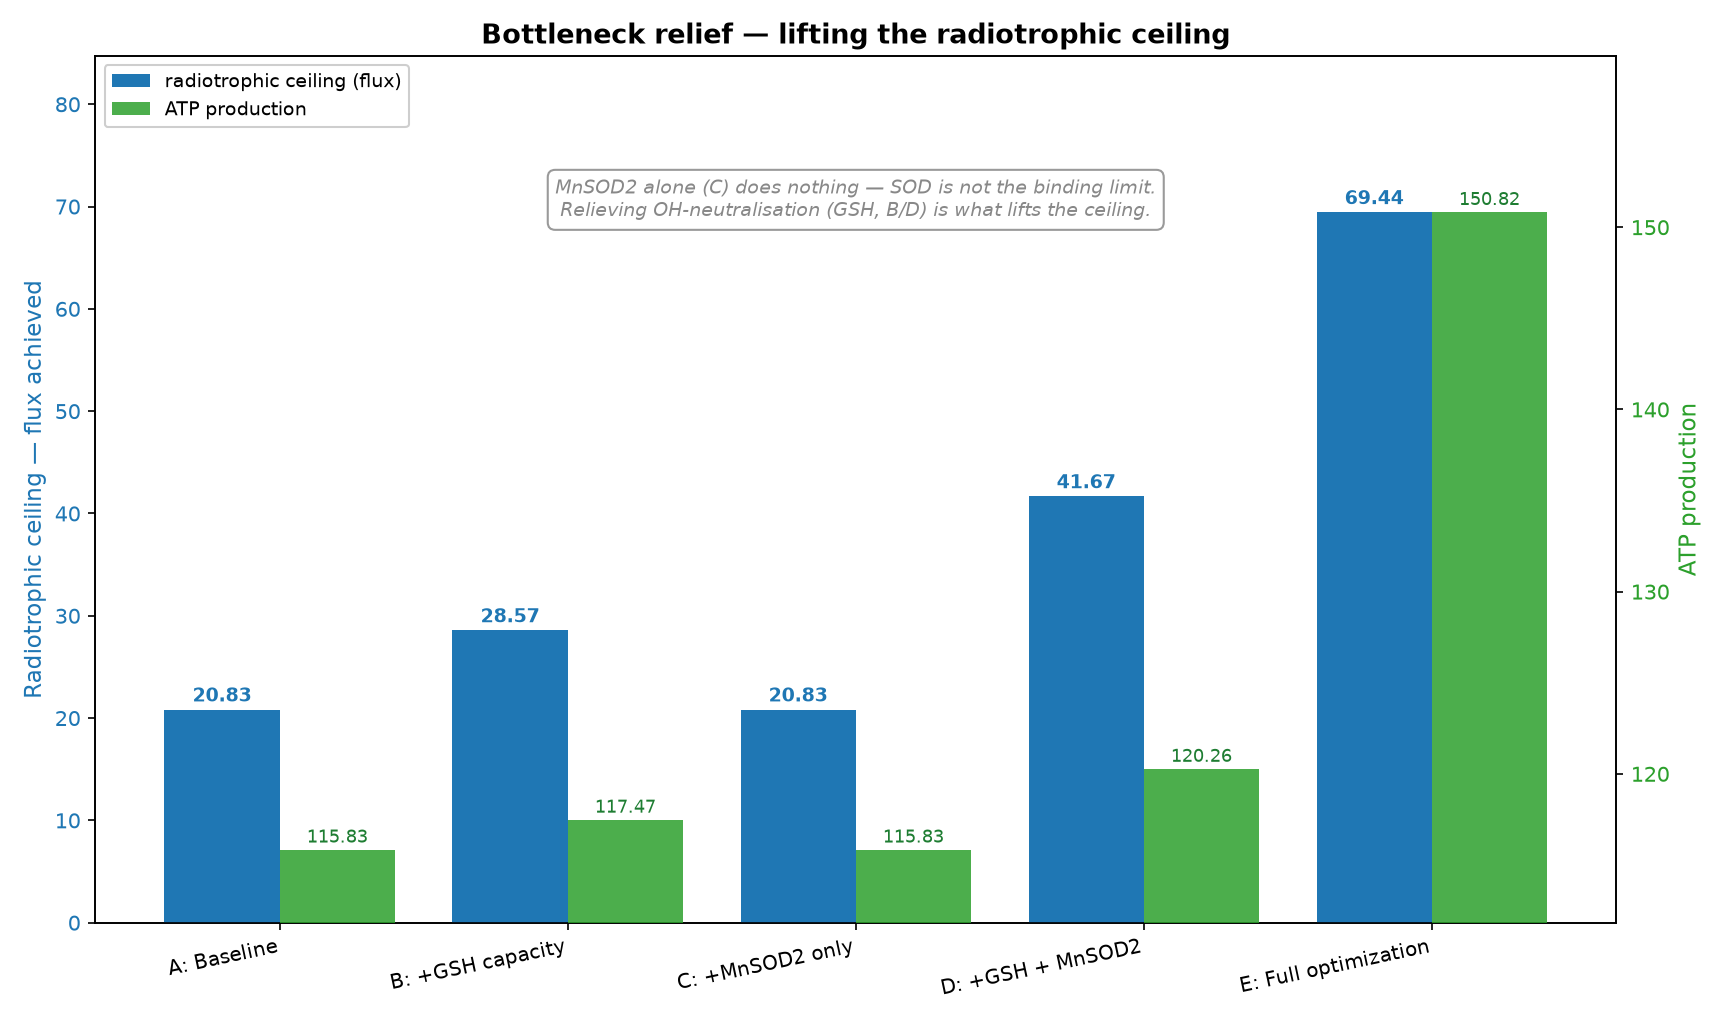
\includegraphics[width=0.92\linewidth]{fig_bottleneck_relief.png}
  \caption{Bottleneck relief. MnSOD2 alone does not raise the ceiling (SOD is not
  the binding limit at baseline); relieving glutathione (OH-neutralization) capacity
  does. Relieving both ROS bottlenecks together, plus synthetic melanin loading,
  lifts the ceiling further.}
  \label{fig:bottleneck}
\end{figure}

\begin{figure}[t]
  \centering
  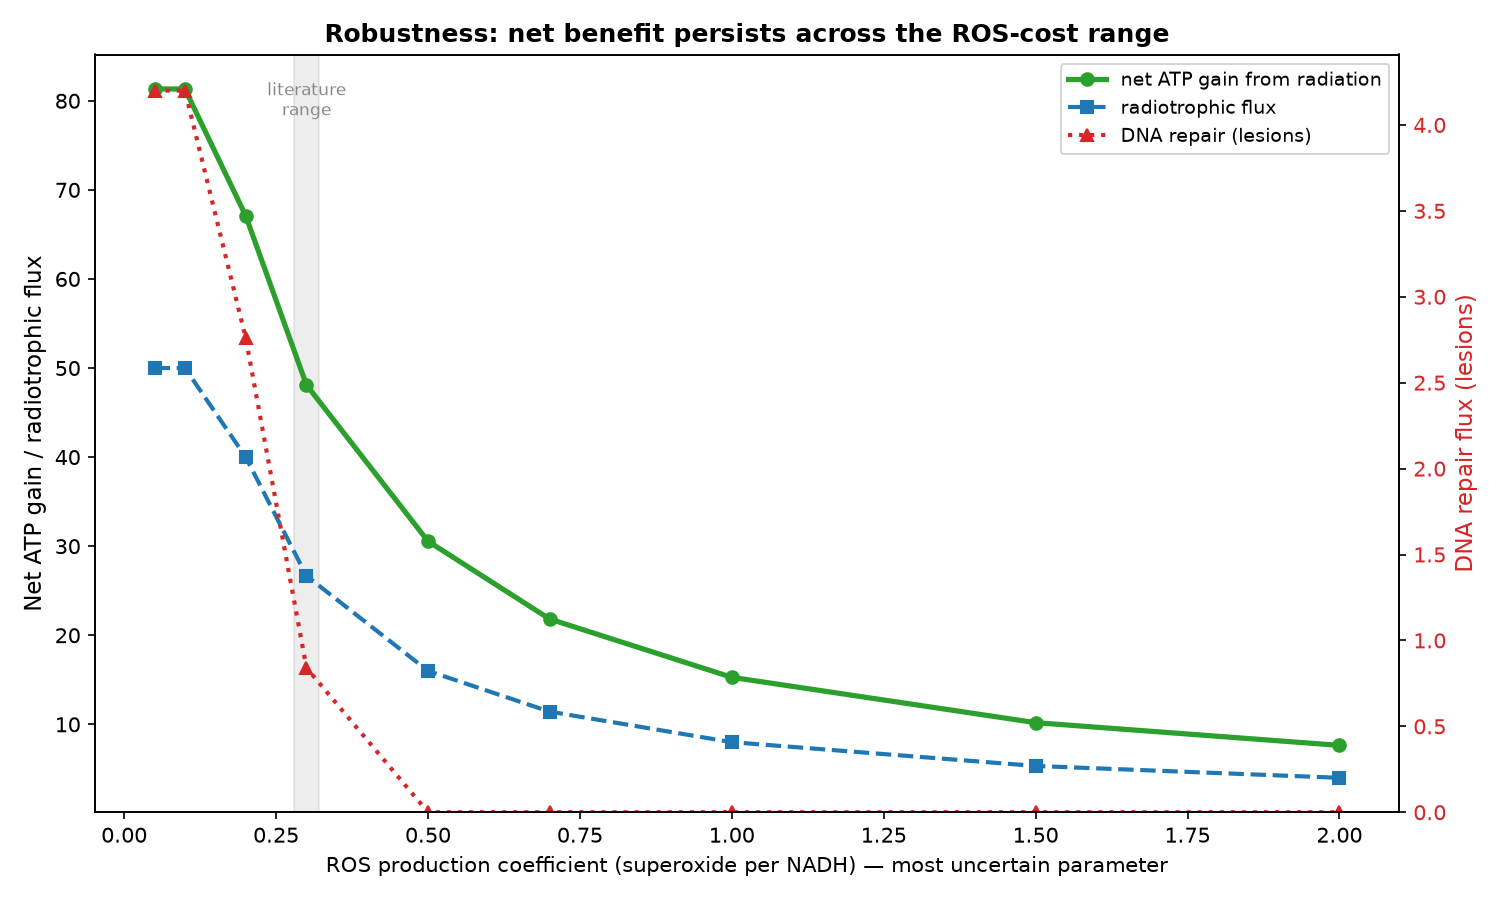
\includegraphics[width=0.92\linewidth]{fig_ros_sensitivity.png}
  \caption{Robustness. Net ATP gain from radiation remains positive across a
  40-fold range of the superoxide-per-NADH coefficient, the most uncertain
  parameter, including the literature-derived band. DNA lesions appear only at the
  low-cost (high-flux) end.}
  \label{fig:ros}
\end{figure}

% ---------------- TABLES ----------------

\begin{table}[t]
  \centering
  \small
  \caption{Cross-species gene-transfer feasibility. Dsup component scores
  (structural compatibility, functional expression, protection efficacy,
  engineering feasibility) give an overall 8.25/10.}
  \label{tab:genes}
  \begin{tabular}{@{}p{3.6cm}p{3.4cm}cl@{}}
    \toprule
    \textbf{Gene / system} & \textbf{Function} & \textbf{Human-tested} &
    \textbf{Feasibility} \\
    \midrule
    Dsup (tardigrade) & DNA protection from OH radicals & Yes & HIGH \\
    Mn-antioxidant (\textit{D.\ radiodurans}) & Protein protection via Mn$^{2+}$ &
    No & MEDIUM \\
    Nrf2 overexpression & Enhanced antioxidant expression & Yes & HIGH \\
    Melanin synthesis (tyrosinase) & Radiation energy capture & Yes & HIGH \\
    \bottomrule
  \end{tabular}
\end{table}

\begin{table}[t]
  \centering
  \small
  \caption{Model predictions versus published experimental observations, evaluated
  against the tolerance-and-capture thesis (not fungal boost magnitude).}
  \label{tab:validation}
  \begin{tabular}{@{}p{4.3cm}p{2.6cm}p{4.6cm}@{}}
    \toprule
    \textbf{Observation} & \textbf{Source} & \textbf{Agreement} \\
    \midrule
    Melanized growth boost under radiation & Dadachova 2007 &
    Supports thesis: radiation is a usable input, not pure damage \\
    ATP decrease in melanized cells, high dose & Bryan 2011 &
    Consistent: matches the STRAINED-to-LETHAL transition \\
    Dsup reduces DNA damage approximately 40\% & Hashimoto 2016 &
    Imposed directly as a 40\% interception cap \\
    \textit{Cladosporium} approximately 21\% ISS growth & Shunk 2022 &
    Same order as the model stress-condition benefit \\
    MnSOD2 enhances radiosurvival & Kolesnikova 2023 &
    Consistent: SOD augmentation raises the survivable dose \\
    \bottomrule
  \end{tabular}
\end{table}

\section*{Data and code availability}

All model code, experiment scripts, generated data, figures, the dose-calibration
module, the test suite, and the wet-lab validation proposal are available in the
project repository.

% ---------------- REFERENCES ----------------

\begin{thebibliography}{99}
\small
\bibitem{bryan2011} Bryan R. et al. (2011) Melanin and radiation tolerance.
\textit{Fungal Biology} 115:945.
\bibitem{buxton1988} Buxton G.V. et al. (1988) Critical review of rate constants
for radiolysis of water. \textit{J. Phys. Chem. Ref. Data} 17:513.
\bibitem{chavez2019} Chavez C. et al. (2019) The tardigrade damage suppressor
protein binds to nucleosomes. \textit{eLife} 8:e47682.
\bibitem{dadachova2007} Dadachova E. et al. (2007) Ionizing radiation changes the
electronic properties of melanin. \textit{PLoS ONE} 2:e457.
\bibitem{daly2004} Daly M.J. et al. (2004) Accumulation of Mn(II) in
\textit{Deinococcus radiodurans}. \textit{Science} 306:1025.
\bibitem{hashimoto2016} Hashimoto T. et al. (2016) Extremotolerant tardigrade
genome and improved radiotolerance via Dsup. \textit{Nature Communications}
7:12808.
\bibitem{kolesnikova2023} Kolesnikova et al. (2023) SOD2 and radiosurvival in
HEK293T. PMC10744337.
\bibitem{lewis2015} Lewis K.N. et al. (2015) Regulation of Nrf2 signaling.
\textit{PNAS} 112:3722.
\bibitem{lindahl2000} Lindahl T., Barnes D.E. (2000) Repair of endogenous DNA
damage. \textit{Cold Spring Harb. Symp. Quant. Biol.} 65:127.
\bibitem{schweitzer2009} Schweitzer A.D. et al. (2009) Physico-chemical evaluation
of melanin for radioprotection. \textit{Int. J. Radiat. Oncol. Biol. Phys.}
73:1494.
\bibitem{shunk2022} Shunk G.K. et al. (2022) Melanized fungal growth on the ISS.
\textit{Frontiers in Microbiology}.
\bibitem{turick2011} Turick C.E. et al. (2011) Gamma radiation interacts with
melanin. \textit{Bioelectrochemistry}.
\end{thebibliography}

\end{document}
